\section{Auswertung}
\label{sec:Auswertung}
\subsection{Nullrate}
\label{sec:Nullrate}
Vor der eigentlichen Messung wird die Nullrate bestimmt. Um den statistischen Fehler möglichst gering zu halten,
wird für eine Zeit von $t=500\,\unit{\second}$ gemessen. Bei dieser Messzeit ergibt sich eine Zählrate von
$N=150$. Die Nullrate bestimmt sich dadurch zu $N_{\symup{u}}=3$ pro $10\,\unit{\second}$ oder zu
$N_{\symup{u}}=9$ pro $30\,\unit{\second}$. Im Folgenden wird die Nullrate immer von den Messwerten abgezogen.

\section{Vanadium}
\label{sec:Vanadium}
Über einen Zeitraum von $t=900\,\unit{\second}$, der in Zeitintervalle von $\Delta t = 30\,\unit{\second}$
aufgeteilt wurde, wurden die in \autoref{tab:vanadium} zu findenden Werte abzüglich der Nullrate gemessen.
\begin{table}
  \centering
  \begin{tabular}{c c}
    \toprule
    Messzeit $t/\unit{\second}$ & Zählrate $N$\\
    \midrule
     30 & 131 \\
     60 & 116 \\
     90 & 122 \\
    120 &  88 \\
    150 &  91 \\
    180 &  72 \\
    210 &  81 \\
    240 &  63 \\
    270 &  58 \\
    300 &  40 \\
    330 &  57 \\
    360 &  36 \\
    390 &  40 \\
    420 &  40 \\
    450 &  49 \\
    \bottomrule
  \end{tabular}
  \begin{tabular}{c c}
    \toprule
    Messzeit $t/\unit{\second}$ & Zählrate $N$\\
    \midrule
    480 &  28 \\
    510 &  19 \\
    540 &  29 \\
    570 &  28 \\
    600 &  19 \\
    630 &   9 \\
    660 &  22 \\
    690 &  13 \\
    720 &  12 \\
    750 &  12 \\
    780 &  12 \\
    810 &  12 \\
    840 &   6 \\
    870 &   9 \\
    900 &   5 \\
    \bottomrule
  \end{tabular}
  \caption{Zählrate für Vanadium.}
  \label{tab:vanadium}
\end{table}
Diese Zählrate $N$ wird in halblogarithmisch gegen die Zeit $t$ aufgetragen.

\begin{figure}
  \centering
  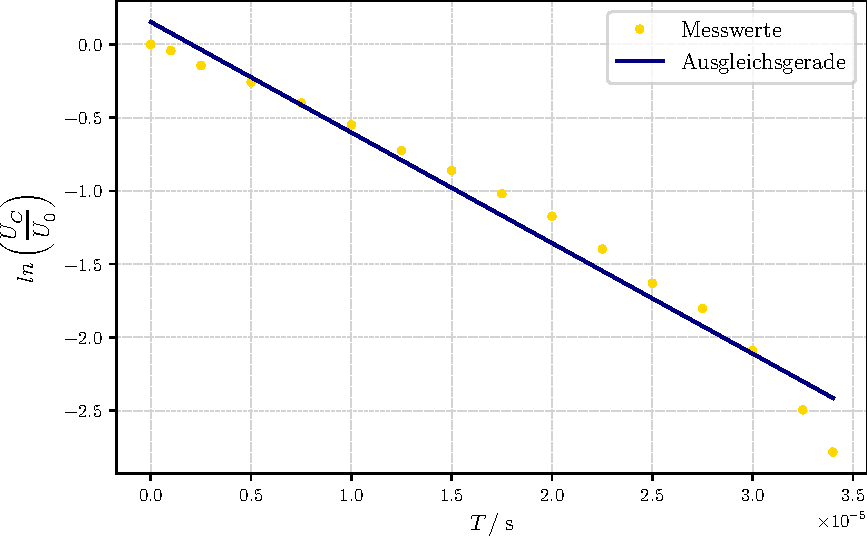
\includegraphics{plot1.pdf}
  \caption{Plot.}
  \label{fig:plot}
\end{figure}